\documentclass[10pt,a4paper]{article}
\let\vec\vec
\usepackage[utf8]{inputenc}
\usepackage{amsmath,amssymb,amsfonts}
\usepackage{natbib}
\textwidth 440pt
\textheight 680pt
\voffset -50pt
\parindent 0pt
\oddsidemargin 20pt
\usepackage{url,hyperref}
\usepackage{graphicx}
\usepackage{subfig}

% journal shorthand
\newcommand\aj{AJ}                   	% Astronomical Journal (the)
\newcommand\mnras{MNRAS}    % Monthly Notices of the Royal Astronomical Society
\newcommand\aap{A\&A}              % Astronomy and Astrophysics
\newcommand\apjs{ApJS}               % Astrophysical Journal, Supplement
\newcommand\apj{ApJ}                 % Astrophysical Journal
\newcommand\nat{Nature}              % Nature
\newcommand\araa{ARA\&A}             % Annual Review of Astronomy and Astrophysics
\newcommand\aapr{A\&ARv}             % Astronomy and Astrophysics Review (the)
\newcommand\pasa{Publ. Astron. Soc. Australia}
\newcommand\aaps{AAPS}
\newcommand\apjl{ApJL}
\newcommand\memras{MmRAS}
\newcommand\pasp{PASP}
\newcommand\nar{New~Astron.~Rev.}

\providecommand{\e}[1]{\times10^{#1}}
\begin{document}

\title{{\bf DRAFT 2:} section 1.2 - Radio Galaxies }
\author{S. Kolwa}
\maketitle

\section{The Birth of Radio Astronomy}\label{section:early-radio-surveys}
The development of the first radio telescopes and surveys are responsible have led to our present understanding of radio galaxies. Many note that radio astronomy began with a serendipitous discovery made by an employee of Bell Telephone Labs, New Jersey in the U.S. While investigating the effect of thunderstorms on transcontinental communication, Karl Guthe Jansky's radio receiver detected a static hiss that appeared to originate from the same location in the sky every 24 hours. The signal would be detected once every sidereal day (four minutes prior to the end of the solar day). This led Jansky to postulate that the source of the signal was non-terrestrial in origin. The signal, detected at a frequency of $\nu_{\rm obs} = 20.5$ MHz ($\lambda_{\rm obs} = 14.6$m), led to him publishing a report on the finding entitled {\it Electrical Disturbances Apparently of Extraterrestrial Origin} - arguably one of the most important papers published on the subject of radio astronomy \citep{Jansky1933b,Jansky1933a}.

In 1937, Grote Reber, a radio engineer and also an avid fan of Jansky went on to construct a 9.5 m paraboloid antenna radio receiver sensitive to $\nu_{\rm obs} = 160$ MHz ($\lambda_{\rm obs} = 1.9$m) radiation which was capable of detecting radio signals from the nucleus of the Milky Way, Sagitarrius A* \citep{Reber1940}. Other discoveries that followed in the wake of this were those of the famous supernova remnants Cassiopeia A, Puppis A and the radio galaxy, Cygnus A. In 1944, Reber completed the first ever radio survey which covered a portion of the northern sky shown in Fig. \ref{fig:Reber-map-sky-1944} \citep{Reber1944}. 

\begin{figure}[!ht]
     \centering
     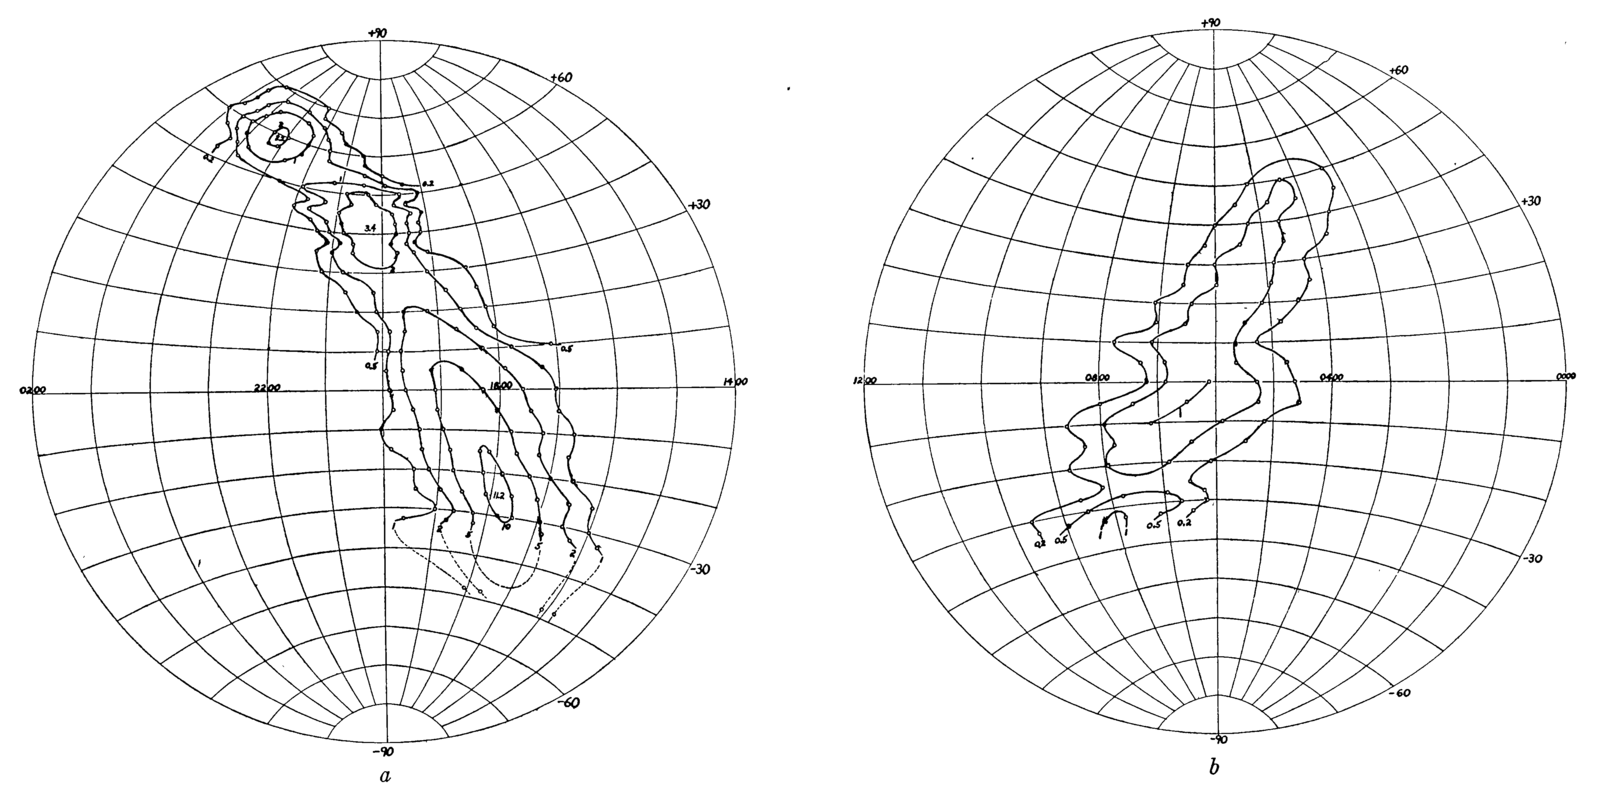
\includegraphics[width=0.8\textwidth]{plots_chp1/Reber_radiomap_1944.png}
     \caption{Intensity contour lines of $\nu_{\rm obs} = 160$ MHz radio emission mapped out by Grote Reber on the self-built 9.5 m parabloid radio telescope \citep{Reber1944}.}
     \label{fig:Reber-map-sky-1944}
\end{figure}

Both Jansky discovery and Reber's work were fundamental to introducing the use of radio frequencies in detecting distant objects within the Milky Way and outside of it. Techniques used in astronomy were developed further through the enhancement of radio receiver technologies used during World War II which led to Baade and Minkowski's own discoveries at the Palomar Observatory, Mount Wilson whose observations showed that two of the sources Reber's first survey detected, Cassiopeia A and Puppis A, spatially coincide with diffuse optical emission referred to as `nebulosities' which were also seen to have large velocity dispersions. Furthermore, the disturbed optical morphology of Cygnus A revealed evidence of it being involved in a galaxy merger \citep{BaadeMinkowski1954}. These cross identifications of a radio sources with optical emission proved that the bright, discrete radio signals picked up by radio surveys were not merely `radio stars' but rather galaxies much like the Milky Way that were emitting powerful bursts of radio emission. Consequently, the term `radio galaxy' became introduced into the astronomy lexicon. 

Hence, in order for a radio source to be considered a radio galaxy, it would need to have an optical counterpart. Without an rest-frame optical, ultraviolet (UV) or infrared (NIR) detection, it would be impossible to quantify the redshift. Measuring the shifts of spectral lines at these wavelengths is the primary method for redshift and, therefore, distance estimation. Of course, the distance of a source is needed to convert the observed parameters of a source such as its flux density, surface brightness or projected size to more intrinsic measures such as luminosity and physical scale-size \citep{Moffet1966}. 

% Motivation section serves to answer:
% Why should we study radio galaxies?


\section{Motivation}\label{section:motivation}
% M-sigma relation - black-hole and galaxy co-evolution
The empirical $M$-$\sigma$ relation, introduced in section 1.1, implies that the mass of the central black-hole (M$_\bullet$) of a galaxy is proportional to its velocity dispersion and thus, the M$_\bullet$ increases with the spheroid mass of the galaxy. Hence, radio galaxies, which generally have high stellar masses should also, by way of this empirical relation, host very massive central black-holes. They should also have high bolometric luminosities ($L_{\rm bol.}$) luminosities due to $L_{\rm bol.}$ scaling upward with accretion rate which is increases with the black-hole mass. Hence, the power output of the active galactic nucleus (AGN) at radio frequencies are what yield the high radio luminosities measured from radio-selected AGN that designate them as `radio-loud'. 

% What are the numbers that define cosmology?
In addition to radio galaxies being some of the best laboratories in which to study kinetic-mode of feedback, there are several other reasons why these galaxies, in particular, are crucial to our understanding of how galaxies evolve. They provide an opportunity to test theories in cosmology given their detection during redshift epochs that probe the very distant and early Universe at $z\sim4-6$ \citep{LillyLongair1984,Miley1989,Lacy1994a,
Waddington1999,VanBreugel1999,Jarvis2009,Saxena2018}. Their detection up to these redshifts is important because by $z\sim6,$ the majority of neutral hydrogen that existed in the Universe during the so-called `Dark Ages' has already been ionised through radiation emitted by the first galaxies and quasars. This early period, referred to as the Epoch of Reionisation (EoR), begins some 150 Myr after the Big Bang (at a redshift of $z\sim20$ and continues up to a cosmic time of 1 Gyr ($z\sim6$) \citep{Zaroubi2013}. Thus, the detection of radio galaxies at high redshifts make them good cosmological probes for parametrising the physics of galaxy formation during the early Universe \citep{Fan2006,Banados2018}.  

% How do galaxies grow / aggregate their mass?
Radio galaxies allow us to gain better insight into how galaxies aggregate their mass through star-formation in their formative phases. The brightness of stellar emission from galaxies can determined from optical and near-infrared band magnitudes \citep{GunnOke1975}. In particular, the relation between the brightness of flux measured in the $K$-band (central wavelength: $\lambda_{\rm c}=2.2~\mu$m) which traces redshifted ultraviolet (UV) and optical emission from young stars and redshift show the evolution of flux from stellar emission with cosmic time. This observed relation, when depicted, is frequently called the Hubble $K$-$z$ diagram. Granted that $K$-band magnitudes are detectable to redshifts of up to $z<4,$ the empirical $K$-$z$ relation for ensembles of radio sources can be used to test cosmology and galaxy evolution models  \citep{LillyLongair1984,EalesRawlings1996,Eales1997}. More recently, the work of \citet{Inskip2002} showed that the $K$-$z$ relation for a sample of radio galaxies fits reasonably to an Einstein-de Sitter cosmology model for a matter density ($\Omega_{\rm M}$) and dark energy density ($\Omega_\Lambda$) of ($\Omega_{\rm M}=1, \Omega_\Lambda=0$). Evidently, the $K$-$z$ diagram has been instrumental in determining the validity of cosmological models.

\begin{figure}[!ht]
    \centering
    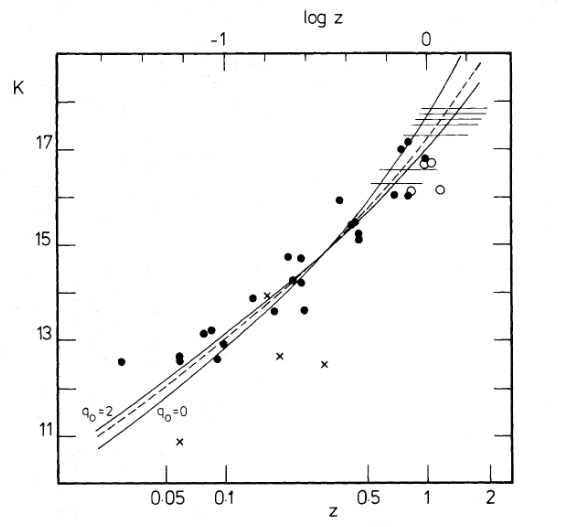
\includegraphics[width=0.8\textwidth]{plots_chp1/K_z_Lill1982.png}
    \caption[Near-infrared Hubble $K$-$z$ diagram \citep{LillyLongair1982}]{Infrared Hubble $K$-$z$ relation from \citet{LillyLongair1982}. The predicted evolution of this relation is shown for cosmological deceleration parameters $q_0=0$ and $q_0=2$ against the observed magnitudes.}
    \label{fig:K-z-Lilly1984}
\end{figure}

It follows that the $K$-$z$ diagram has become a widely used diagnostic for placing constraints on galaxy evolution models given that it is a tightly constrained empirical relation, with a low level of scatter and therefore reliable. The work of \citet{rocca-volmerange2004} make use of the $K$-$z$ diagram to predict the stellar masses of radio galaxies. In this work, the apparent (observed) $K$-band of an ensemble of radio galaxies compiled by \citet{deBreuck2002} that were first detected in the 3CR and 6CE catalogues discussed in section \ref{section:early-radio-surveys}. The galaxies are detected over the redshift range $0 \leq z \leq 4$ and are shown against galaxy evolution models which predict the baryonic masses of elliptical galaxies as shown by Fig. \ref{fig:K-z-rocca-volmerange2004-pegase}. For the radio galaxies, the results suggested that their baryonic masses ($M_{\rm bary.}$) should lie within the range, $10^{11} < M_{\rm bary.}/\rm{M}_\odot < 10^{11.5}.$ They also reveal a general upper limit of $M_{\rm bary.}/\rm{M}_\odot < 10^{12}$ for all galaxies implying that radio galaxies are the most massive galaxies detectable, in terms of their baryon masses.

\begin{figure}[!ht]
  \centering
  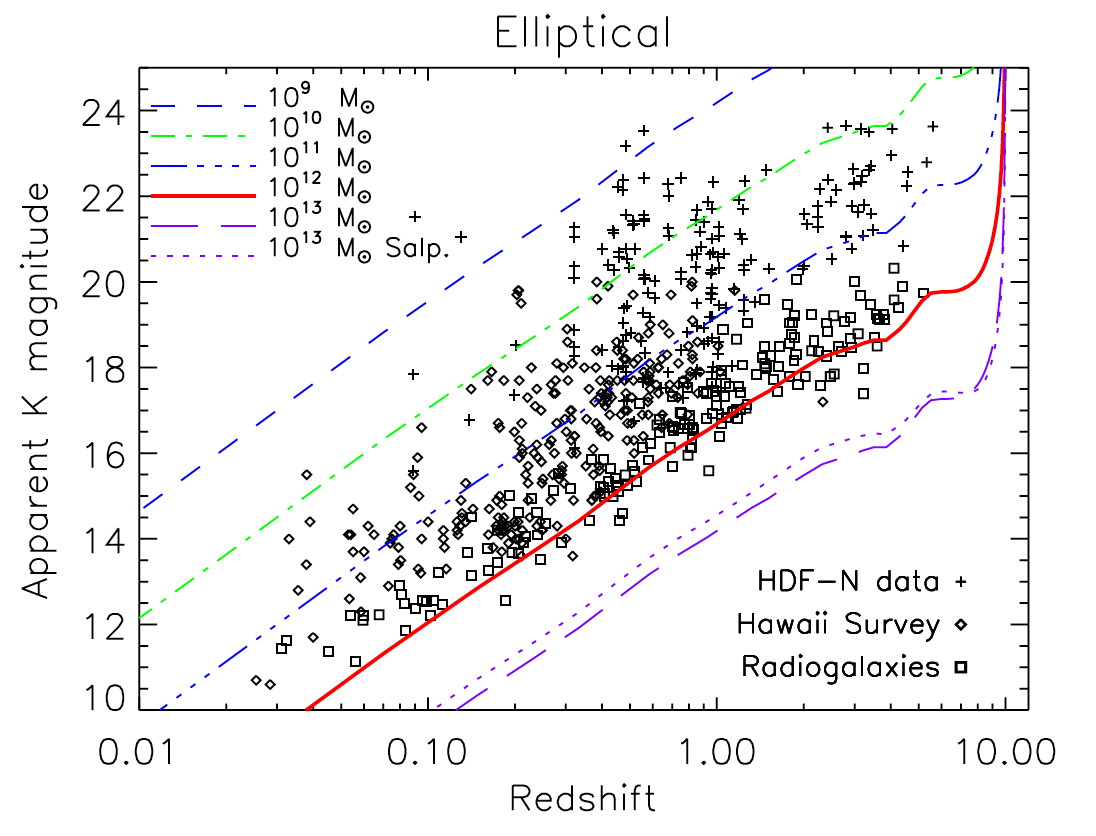
\includegraphics[width=0.8\textwidth]{plots_chp1/K_z_Rocca-Volmerange_2004_pegase.png}
  \caption{The $K$-$z$ diagrams of radio galaxies (squares) from 3CR and 6CE. The data also includes K-band magnitudes of field galaxies from the Hawaii Survey \citep{Songaila1994} (diamonds) and HDF-N \citep[Hubble Deep Field-North;][]{Dickinson2003} (crosses). The initial mass function (IMF) models from \citet{RanaBasu1992} which are given for a range of baryonic masses from $M_{\rm bary.} = 10^9 - 10^{13}$ M$_\odot.$ A top-heavy (TH) IMF model for $M_{\rm bary.} = 10^{13}$ M$_\odot$ is included for comparison.}
  \label{fig:K-z-rocca-volmerange2004-pegase}
\end{figure}

The predicted range of radio galaxy baryonic masses from \citet{rocca-volmerange2004} are in agreement with those predicted by \citet{seymour2007} who made use of data from the {\it Spitzer Space Telescope} (SST) \citep{Werner2004}. The dataset comprises SST near-IR photometry for 69 radio galaxies between redshifts of $1.0 < z < 5.2.$ The {\it Spitzer} photometry obtained by the instruments on board the telescope namely the Infrared Array Camera (IRAC; $3.6-8.0~\mu$m), Infrared Spectrograph (IRS; 16 $\mu$m) and Multi-band Imaging Photometer (MIPS; $24-160~\mu$m). Spectral energy distribution (SED) models that aimed to disentangle the stellar, dust and AGN components within the optical and near-IR emission were fit to the data as well as obtain stellar masses from $H$-band magnitudes (at a central wavelength of $\lambda_{\rm c} = 1.65$ $\mu$m)\footnote{The choice to use $H$- rather than $K$-band magnitudes is motivated by galaxy evolution models which show that the predicted flux of radio galaxies peaks at the central wavelength of the $H-$band. Additionally, SED-fitting in \citet{Drouart2012} showed that $H-$band is optimal for sampling the stellar mass without too much contamination from heated dust emission.}. The result of this study shows that the radio galaxies have stellar masses (M$_*$) within the range of $10^{11} < M_* < 10^{11.5}$ M$_\odot.$ Studying radio galaxies thus permits us to determine what drives the formation and evolution of galaxies with irregularly high stellar masses. 

% How are jets formed?
Observations generally give us with an incredible wealth of information concerning the physical processes that occur within radio galaxies. Although they provide a real-world view of astrophysical objects as they existed, with the caveat of observational biases include, they only provide snapshots of the object at a given epoch. A simulation, although controlled by man not nature, provides us with a continuous and evolving view of a galaxy. Hydrodynamical simulations have provided a simulated view of radio jets and the impact they bear on the surrounding gas medium through which they propagate. This has been done by \citet{krause2002} and \citet{krause2005} who demonstrate that shells of neutral hydrogen gas, responsible for Ly$\alpha$ absorption in high redshift radio galaxies, can form at the bow shock fronts of radio jets through shock-driven compression of gas. Given sufficient time (over Gyr timescales), the neutral hydrogen shells can subsequently be shredded at the shock front due to Rayleigh-Taylor instabilities being induced into the neutral gas medium. 

Another instance of radio jet simulations is shown by the Monte Carlo 1D simulations from \citet{Gaibler2011}. Here, radio jets are simulated to propagate into a clumpy interstellar medium (ISM). Snapshots of the simulation, shown in Fig. \ref{fig:jet-ism-Gaibler2011}, illustrate the impact of radio jets on the surrounding gas medium at three different moments during the duty cycle of the radio jet. The average duty cycle of radio jet activity persists over a time-scale of $\tau_{\rm jet} \simeq 10 - 100$ Myr. Simulations of jet-gas interactions indeed suggest that radio galaxies are prime targets for understanding the impact that radio jets have on the gas within the ISM that lies in proximity to an AGN.

\begin{figure}[!ht]
  \centering
  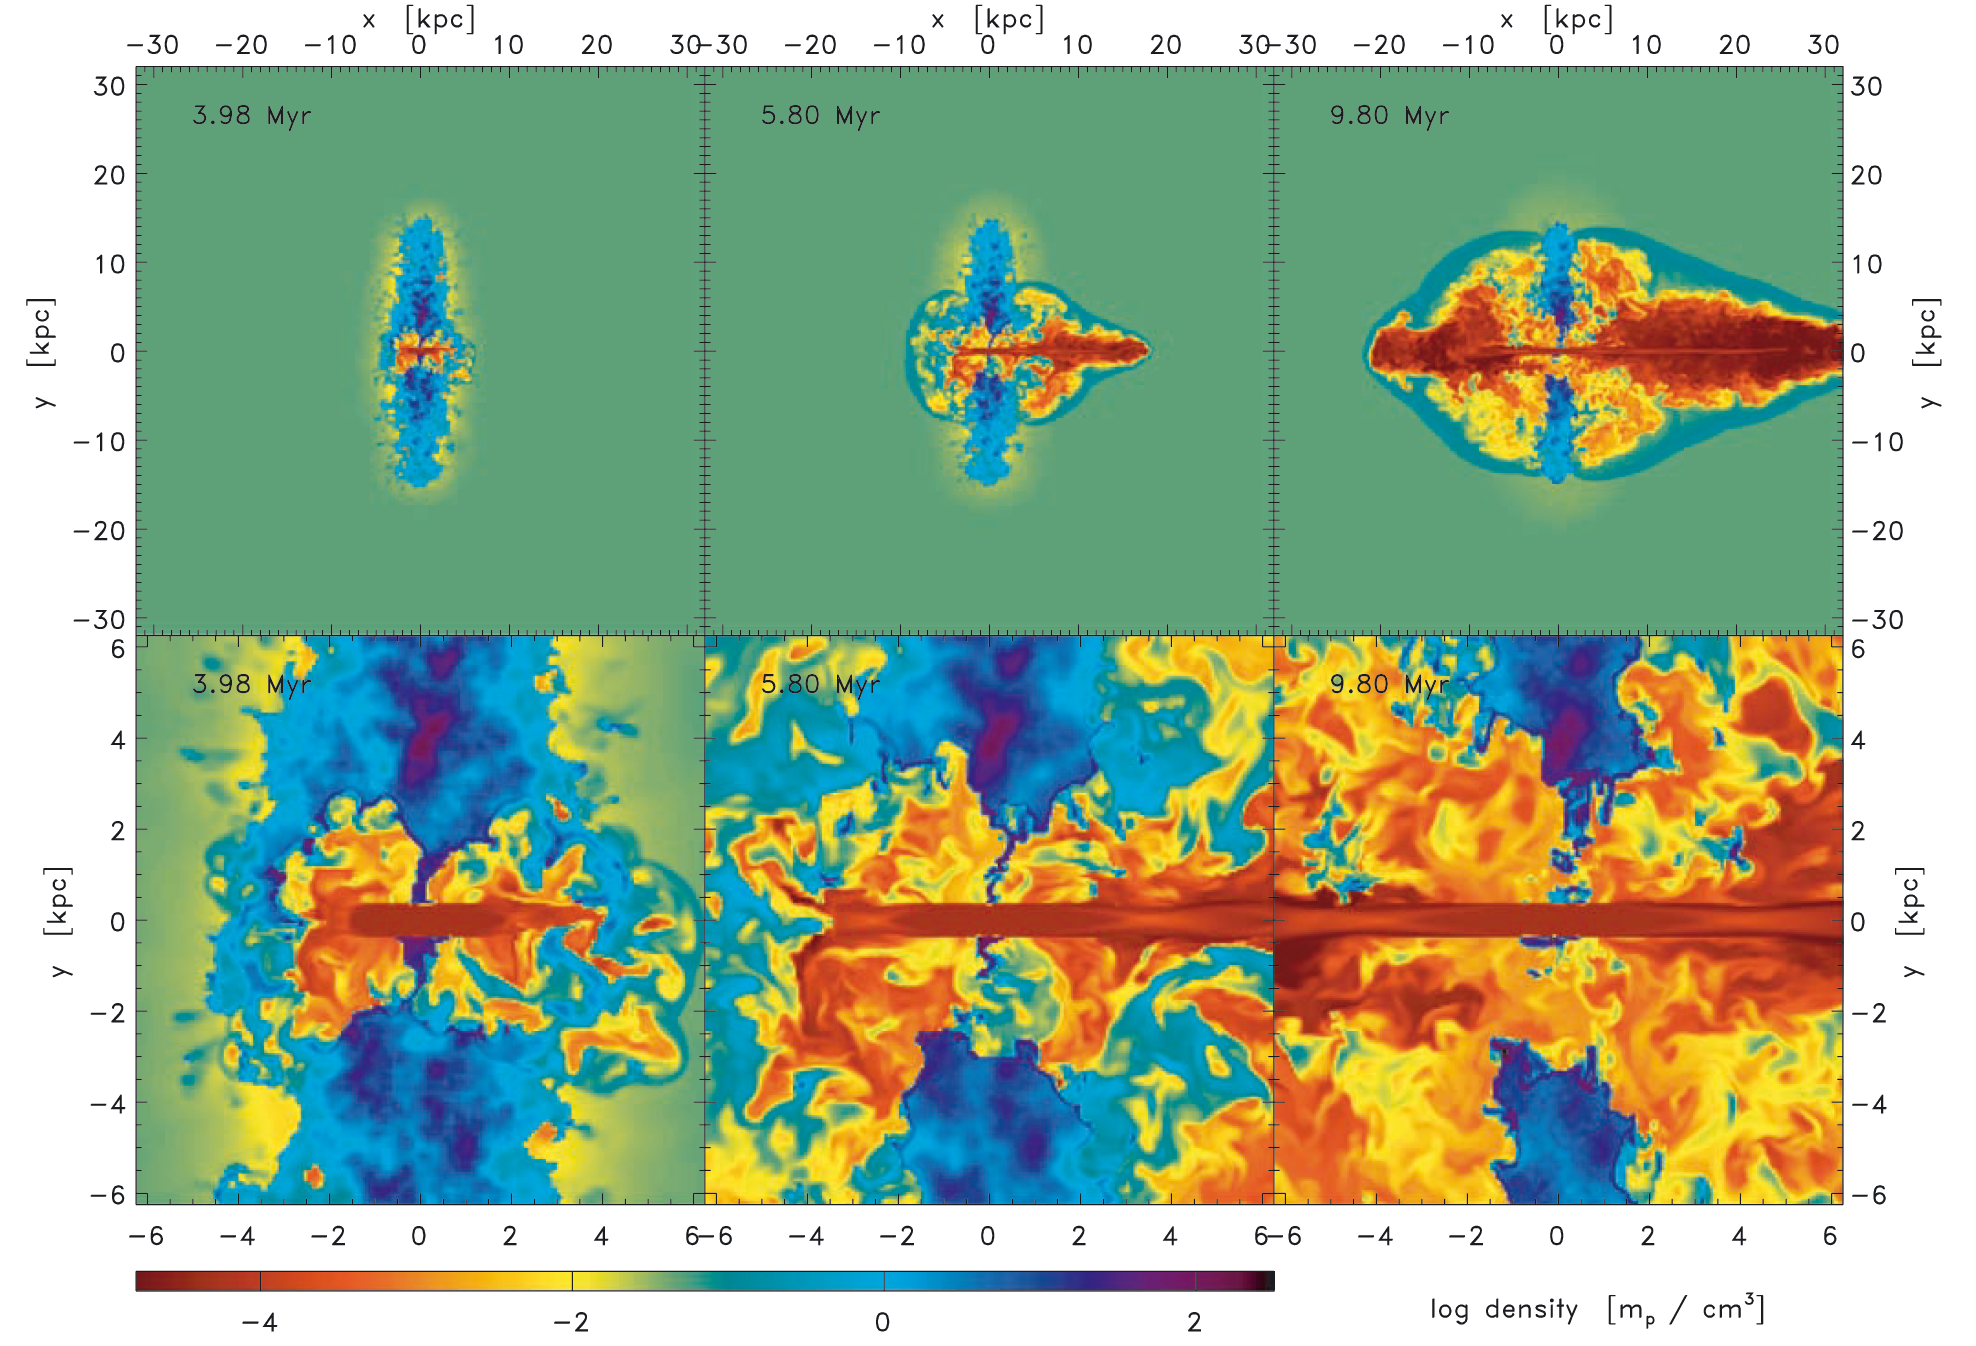
\includegraphics[width=\textwidth]{plots_chp1/jet_gas_sims_Gaibler_2011.png}
  \caption[Simulation snapshots of biconical radio jet from \citet{Gaibler2011}]{Snaphots of 1D Monte Carlo simulations of a biconical radio jet pummelling through a disc-shaped clumpy interstellar medium with log-normal density distribution in \citet{Gaibler2011}. The growing radio jet begins to plough through the clumpy ISM medium at $t=3.98$ Myr. At $t=5.80$ Myr, an asymmetry in the lobes formed by the relativistic jets has already formed. After $t=9.8$ Myr has passed (the average duty cycle of a radio AGN), extended asymmetric radio lobes enclosed in a bow shock region are apparent. The upper panel shows a large-scale view of the simulation with the lower zooming in on the core activity.}
  \label{fig:jet-ism-Gaibler2011}
\end{figure}

% How could kinetic-mode of feedback affect SF ? 
Radio galaxies at high redshifts are known to form stars rapidly with star-formation rates (SFR) of $\rm SFR \gtrsim 100 - 1000$ M$_\odot \rm yr^{-1}$ inferred from SED fitting to near-IR photometry \citep{Drouart2014,Falkendal2019}. The resulting SFR and black-hole accretion rates inferred from the SED-fitting are plotted in Fig. \ref{fig:SFR_AGN_LIR}. These SFR together with the M$_*$ of HzRGs are sufficient to determine the $\Delta$(M.S.) (shift from the Main Sequence) of the galaxies. The Main Sequence of star-forming galaxies defines the expected SFR for a galaxy with a given stellar-mass. The placement of the \citet{Falkendal2019} HzRG sample is shown against the Main Sequences of star-forming galaxies in Fig. \ref{fig:HzRGs-MS-Falkendal2019}. What is clear from these plots, is that at $z > 3,$ more of the HzRGs are found below the Main Sequence. This implies that, although HzRGSs form stars rapidly, their SFR are not rapid enough to account for their masses at $z > 3.$ At later epochs, $ 1.3 < z < 3,$ the HzRGs tend to fall along the Main Sequence. Therefore, HzRGs appear to have be in the process quenching or undergoing a fast decrease in star-formation by $z\sim3.$ This effect may be due to AGN jet feedback that is driving outflows of molecular gas which fuels star-formation. Once more, proving how critical radio galaxy studies in understanding the effects of radio jets on the evolution of galaxies. 


\begin{figure}[!ht]
    \centering
     \subfloat[The total AGN luminosity, $L^{\rm IR}_{\rm AGN}$ as a function of the star-forming luminosity $L^{\rm IR}_{\rm SF}$ from \citet{Drouart2014}. The top axis converts $L^{\rm IR}_{\rm SB}$ to SFR using the \citet{Kennicutt1998} relation. The right axis converts $L^{\rm IR}_{\rm AGN}$ to $\dot{M}_{\rm BH}$ assuming $\epsilon=0.1$ and $\kappa^{\rm Bol}_{\rm AGN}.$ The dashed line marks $L^{IR}_{AGN} = L^{\rm IR}_{SB}.$ This dashed line indicates the relation corresponding to $\dot{M}_{\rm BH} = 0.024 \times \rm SFR,$ using the right and top axes. The dotted line represents the parallel growth mode, where black holes and galaxies grow simultaneously, following the $M_{\rm BH}-M_{\rm Gal}$ relation.]{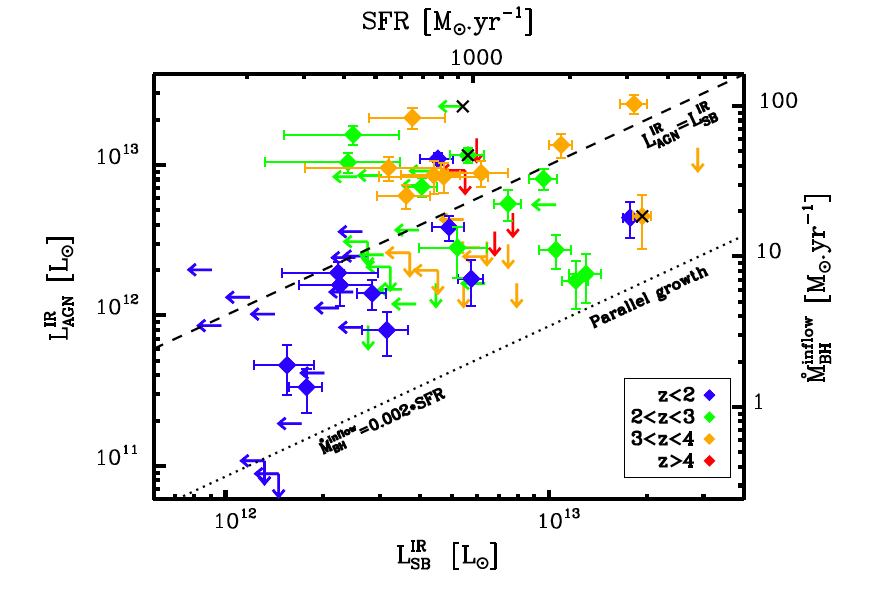
\includegraphics[width=0.9\textwidth]{plots_chp1/SFR_AGN_LIR_Drouart_2014.png}}\\
    \subfloat[$L^{\rm IR}_{\rm AGN}$ as a function of $L^{\rm IR}_{\rm SF}$ from \citet{Falkendal2019}. The dashed black line represents equality between the ordinate and abcissa which also represent the star-formation rate (SFR) and black-hole (BH) mass accretion rate ($\dot{M}^{\rm acc.}_{\rm BH}$). The dotted shows the axis where black-hole accretion rate $\dot{M}^{\rm acc.}_{\rm BH} = 0.002 \times \rm SFR$ which demarcates parallel growth mode where the galaxy and black hole grow in tandem and obey the spheroid mass-BH mass relation.]{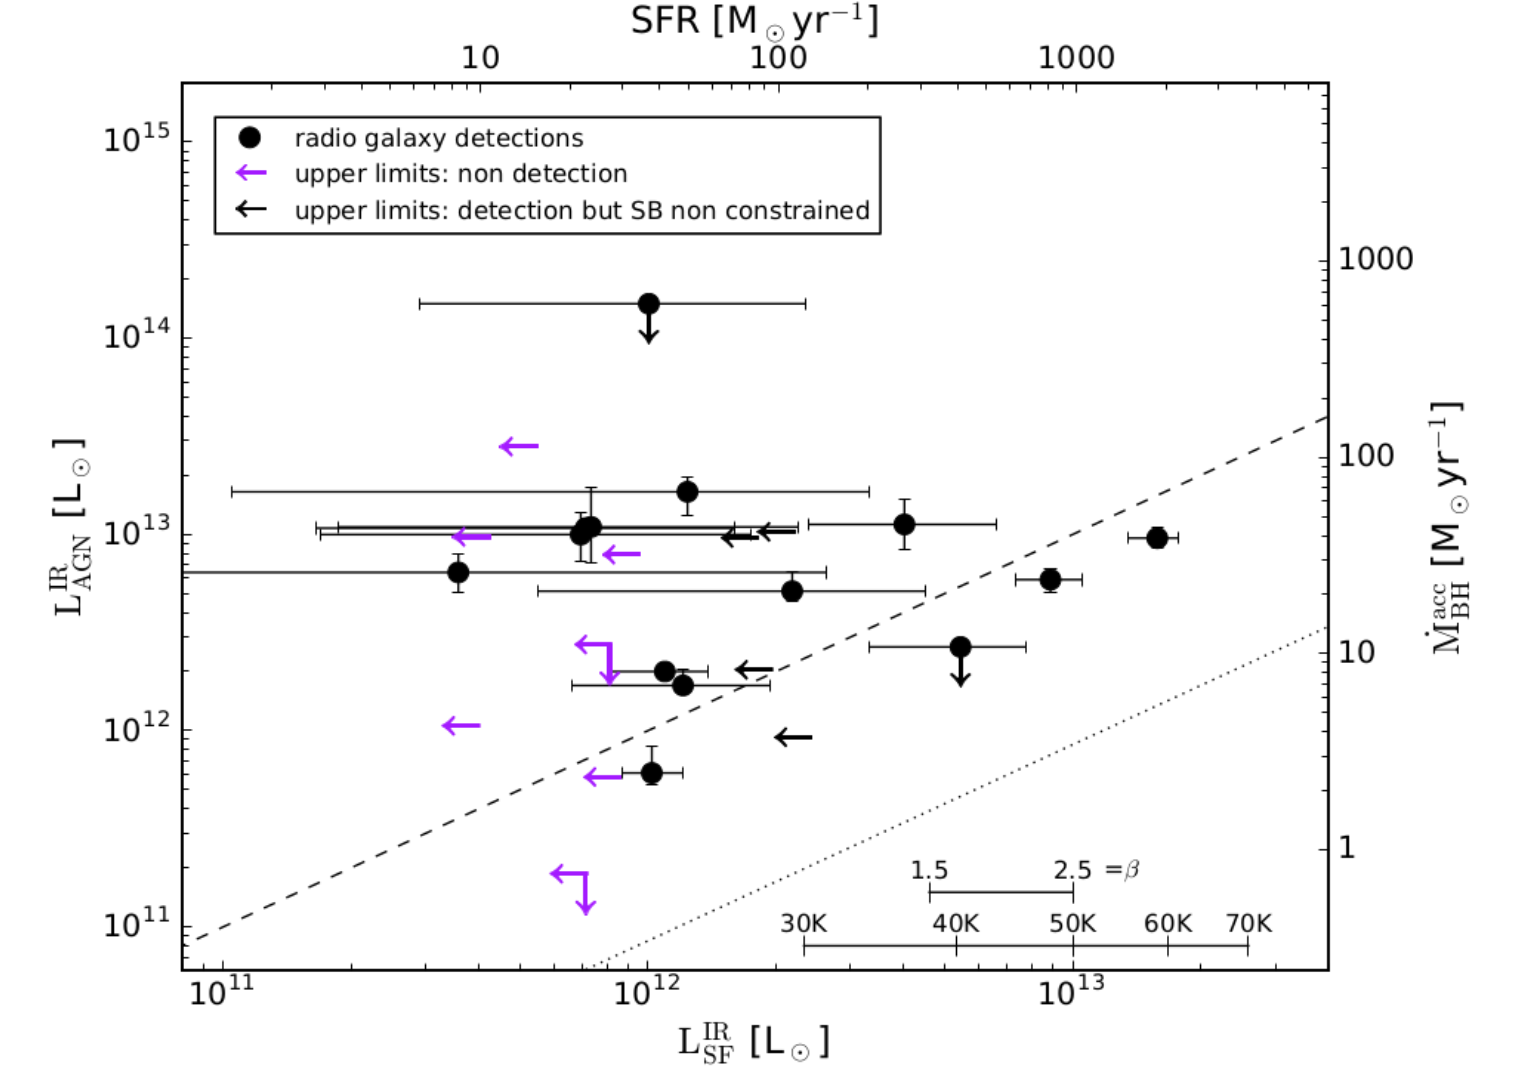
\includegraphics[width=0.75\textwidth]{plots_chp1/SFR_AGN_LIR_Falkendal_2019.png}}
    \caption[AGN vs SF luminosity from \citet{Drouart2014} and \citet{Falkendal2019}]{AGN luminosity, $L^{\rm IR}_{\rm AGN}$ as a function of the star-formation luminosity $L^{\rm IR}_{\rm SF}$ from \citet{Drouart2014} and \citet{Falkendal2019}.}
    \label{fig:SFR_AGN_LIR}
\end{figure}

\begin{figure}[!ht]
   \centering
   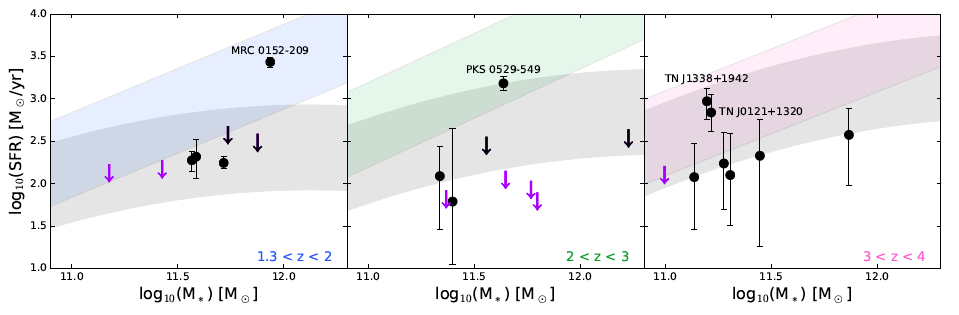
\includegraphics[width=\textwidth]{plots_chp1/HzRGs_main_sequence_Falkendal2019.png}
   \caption[HzRGs relative to Main Sequence in \citet{Falkendal2019}]{HzRGs from \citet{Falkendal2019} sample are compared to the Main Sequences in the grey shaded regions are from \citet{Schreiber2015} while the coloured ones are from \citet{Santini2017}. }
   \label{fig:HzRGs-MS-Falkendal2019}
\end{figure}

The Lilly-Madau plot of the cosmic star-formation rate density (SFRD) is well known in astronomy and presents a rather intriguing puzzle that has been solved, in parts \citep{Lilly1995,Madau1996}. It shows that at $z \simeq 1.9$ (3.5 Gyr after the Big Bang) the level of cosmic star-formation per epoch per volume reaches a peak as Fig. \ref{fig:SFRD_z_Madau_Dickinson2014} illustrates \citep{MadauDickinson2014}. It has been demonstrated that only populations of galaxies that follow the Main Sequence relation can cause this increase in the cosmic SFRD at $1 < z < 3$ therefore HzRGs, which are found on the main sequence at these redshifts, may be important in explaining the function, $\psi(z).$ Unlike, normal main-sequence star-forming galaxies which do, radio galaxies host powerful jets that have a unique impact on the gas that is gravitationally bound to a galaxy and in close proximity to the AGN. Hence, they hold great importance in providing clues about star-formation processes and how it is affected by jet-driven gas outflows. 

\begin{figure}[!ht]
   \centering
   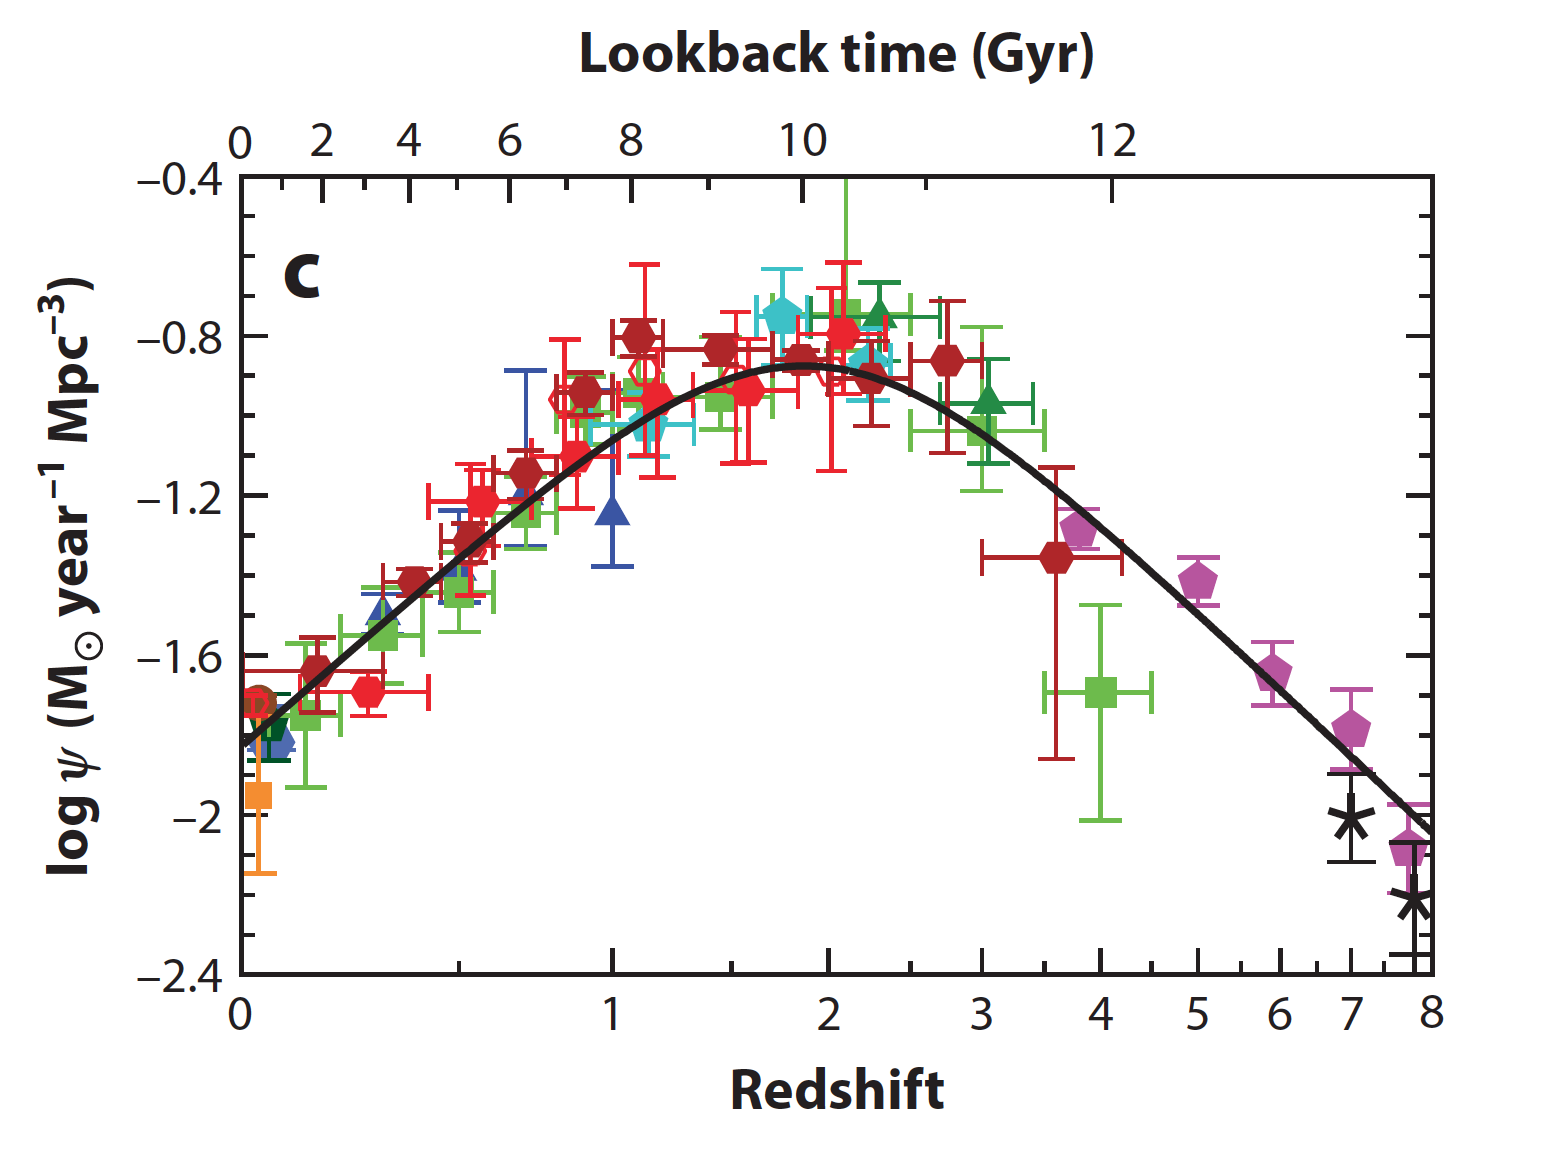
\includegraphics[width=0.8\textwidth]{plots_chp1/SFRD_z_Madau_Dickinson_2014.png}
   \caption[SFRD as a function of redshift in \citet{MadauDickinson2014}]{The star-formation rate density (SFRD) or $\psi$ in M$_\odot$ yr$^{-1}$ Mpc$^{-3}$ given as a function of redshift as well as lookback time in Gyr. The measurements shown are obtained from far ultraviolet (FUV) and near-infrared (NIR) rest-frame luminosities which are converted to SFR. In the FUV, the equation SFR $= \kappa_{\rm{FUV}} \times L_\nu (\rm{FUV})$ while in the NIR, it is obtained via SFR $= \kappa_{\rm{IR}} \times L_{\rm{IR}}.$}
   \label{fig:SFRD_z_Madau_Dickinson2014}
\end{figure}

\section{Radio galaxies across cosmic time} 
\subsection{Early Radio Surveys}
In the wake of pioneering events in radio astronomy such as Jansky's discovery of cosmic noise, Reber's 160 MHz radio survey and Baade and Minkowsi's identification of radio galaxies, a number of radio surveys were successfully completed. The result was, of course, an increase in the number of known radio sources, generally and radio galaxies. 

The Third Cambridge Catalogue \citep[3C][]{Edge1959}, was formed using the Cambridge Inteferometer, is one of first and most prolific. The first and second Cambridge catalogues (1C and 2C) were also compiled in Cambridge in 1950 \citep{Ryle1950} and 1955 \citep{Shakeshaft1955}. Despite being the first Cambridge radio survey catalogues, however, 1C and 2C contained sources affected by astronomical `confusion' which is a consequence of more than one astronomical source being detected within the synthesised beam. The result of this is several sources being incorrectly resolved as one source. and set the stage for identifying a significant number of radio galaxies including the sources 3C 295 which was the most distant radio galaxy known at the time of its discovery \citep{Minkowski1960}. 

The revised 3C Catalogue \citep[3CR][]{Leslie1961,Bennett1962} observed at $\nu_{\rm obs} = 178$ MHz at a sensitivity or flux limit of $S_{178} = 9$ Jy contained a large number of bright sources at declinations, $\delta > -5^{\circ}$ - in the northern hemisphere. A radio interferometer at the Palomar Observatory Sky Survey \citep[POSS][]{Veron1966} identified optical counterparts to a number of 3C sources to accurately calibrate the radio source positions and determine whether the optical and radio detections coincide spatially (are related to the same source). Even further revision of the original 3C source list was carried out by \citet{LaingRileyLongair1983} forming the 3CRR catalogue ($S_{178} \geq 10$ Jy) which contained sources that had yet to be detected due to flux limits of the original 3C survey. 

The more notable catalogues to follow were 4C \citep{PilkingtonScott1965} which was also tuned to an observing frequency of $\nu_{\rm obs} = 178$ MHz at a flux limit of $S_{178} = 2$ Jy. This catalogue was crucial in the identification of sources that had spectral indices $\alpha < -1$ in the flux density-frequency relation, $S_\nu \propto \nu^{-\alpha}$ at tuning frequencies, $\nu > 178$ MHz. This selection bias led to the identification of sources with small angular sizes and high radio luminosities which implied that they were more distant than sources with less steep spectra \citep{Tielens1979}. These distant radio sources formed the 4C Ultra Steep Spectrum Sample \citep[4C/USS][]{ChambersMiley1990} that consists of distant radio galaxies with redshifts of 35 sources at $z > 2$ and 2 at $z > 3.$ The legacy of Cambridge catalogues has continued on through the years all the way on to the most recent, 10C Survey \citep{AMIConsortium2011}. 

The Molonglo Reference Catalogue of Radio \citep[MRC][]{Large1981} 12,141 sources were detected at a tuning frequency of $\nu_{\rm obs} = 408$ MHz at a flux limit of $S_{408} \geq 0.7$ Jy on the Molongolo Radio Telescope \citep{Hunstead1972}. From MRC, steep spectrum sources with $\alpha < -0.9$ were selected at $S_{408} >0.9$ Jy which included accompanying optical long-slit spectroscopy which showed that many of the sources are at redshifts of $z > 0.8$ \citep{McCarthy1990} Further investigations on a subset of MRC sources at $S_{408} >0.95$ Jy revealed several $z > 1$ radio galaxies with extended optical emission structures and more luminous radio cores and jets than 3C sources \citep{McCarthy1991}. 

The efforts made to build up source catalogues from radio interferometric surveys during the early days of radio astronomy have provided an extensive repository of sources at low and high redshifts. Having a wide enough database from which to study the evolution of radio galaxies from their early formation after the Epoch of Reionisation to the local Universe. 

\subsection{Radio galaxies across cosmic time}
As the large-scale structure of the Universe changes with across time through cosmic expansion \citep{Planck2016} so do the properties of galaxies. One of the main goals of this entire thesis, in fact is to compare and contrast the properties of radio-loud AGN host galaxies at high and low redshift. In this section, I highlight some the known commonalities and disparities of these galaxies at the different redshift epochs where they are found.  

Radio galaxies are empirically defined as radio-loud sources that have double-lobed morphologies formed through the expulsion of synchrotron radiation from bipolar (bi-directional) jets emitted from their cores. 
A perfect illustration of this is the nearby galaxy Cygnus A ($z=0.057$), a local radio galaxy first identified by \citet{JennisonDasGupta1953}. Early and more recent interferometric observations shown in Fig. \ref{fig:CygA} clearly exhibit its double-lobed radio structure \citep{Moffet1966,CarilliBarthel1996}. Provided that a radio galaxy is at a sufficiently low-redhsift for its radio structure to be resolved, this morphology will be apparent. High-redshift radio galaxies have lobe structures extended to 100 kpc sizes and are resolved even up to $z \lesssim 4$ \citep{Miley1980,Carilli1997,pentericci1999}.  

The double-lobe morphology implies that the relativistic jets are orientated along the plane. This is important as a radio source classifier. A Type 1 source would have `beamed' jets where the observer stares down the barrel of the radio jet's ionisation code. The Type 2 source refers to the jets being observed parallel to (or at a small angle from) the plane of the sky. Therefore, by definition, all radio galaxies are Type 2 AGNs. Their double-lobe morphologies also put them in the category of Fanaroff-Riley II sources which have extended lobes which terminate at edge-brightened hotspots where enhanced non-thermal radiation at the edge of these radio structures \citep{FanaroffRiley1974}. 

Radio galaxies have classically been dichotomised into radio-loud and quiet populations based on their obsserved radio luminosities. Many of the first studies to identify this bi-modality in radio sources identified the objects as quasars rather than radio galaxies per se or that radio galaxies have quasars hidden by cosmic dust \citep{Vernet2001}. Granted that radio galaxies and quasars may be the same objects viewed at different angles, the empirical definitions of radio-loud and radio-quiet quasars also extend to radio galaxies. 

Generally, the radio-loud sources, which are rarer than radio-quiet ones, have comparatively higher radio luminosities and are hosted by elliptical galaxies \citep{Padovani1993}. Radio-quiet sources on the other hand are not observed in ellipticals \citep{Wilson1995}. Empirically, the lower limit for radio-loud sources can be defined by radio luminosities of $L_{1.4~\rm GHz} \gtrsim 10^{25}$ W Hz$^{-1}$ or $L_{5~\rm GHz} > 10^{26}$ W Hz$^{-1}$ \citep{Miller1990}. More recently, radio luminosity functions of sources in the local Universe have shown that the star-forming galaxy populations that do not form jets at their nuclei outnumber AGN by a factors of up to 10 at $L_{1.4 \rm GHz} < 10^{23}$ W Hz$^{-1}.$ Thus, even though star-forming galaxies may be detectable at radio frequencies, their luminosities tend to be significantly lower than those of radio-loud AGN \citep{Best2005a}. 

How the radio jets are produced is still a matter that largely up for debate. The more widely accepted theory is that they are produced through synchrotron radiation which is emitted as a result of the acceleration of electrons by magnetic fields. The free electrons exist within a plasma surrounding the central black-hole where neutral gas is sufficiently heated and ionised by radiation produced by the AGN. The synchrotron radiation theory was first proposed roughly by \citet{Shklovskii1953} proposed that synchrotron powers relativistic jets which, over Myr time-scales, form the extended lobes that are known to have radio sizes of up to $d\simeq100$ kpc. Given that the sources are radio-loud with luminosities detected in radio frequencies of $L > 10^{25}$ W Hz$^{-1}$ and the average lifetime of a radio source (its duty cycle) falls within a range of $\tau\simeq10-100$ Myr, synchrotron radiation is sufficient to power the radio lobes energies of up to $E \simeq 10^{30} - 10^{40}$ erg over periods of radio AGN activity.

\begin{figure*}[!ht]
  \centering
  \subfloat[The nearby ($d_{\rm L} = 256.3$ Mpc) radio galaxy, Cygnus A, observed with the Cambridge Telescope with a synthesised beam of $23'' \times 35''$ observed at $\lambda=21$ cm. The corresponding radio contours show the double-lobed morphology. The radio contours are superimposed over an optical image taken using the Hale Reflector Telescope. The optical image has a $4' \times 6'$ wide field-of-view \citep{Moffet1966}.]{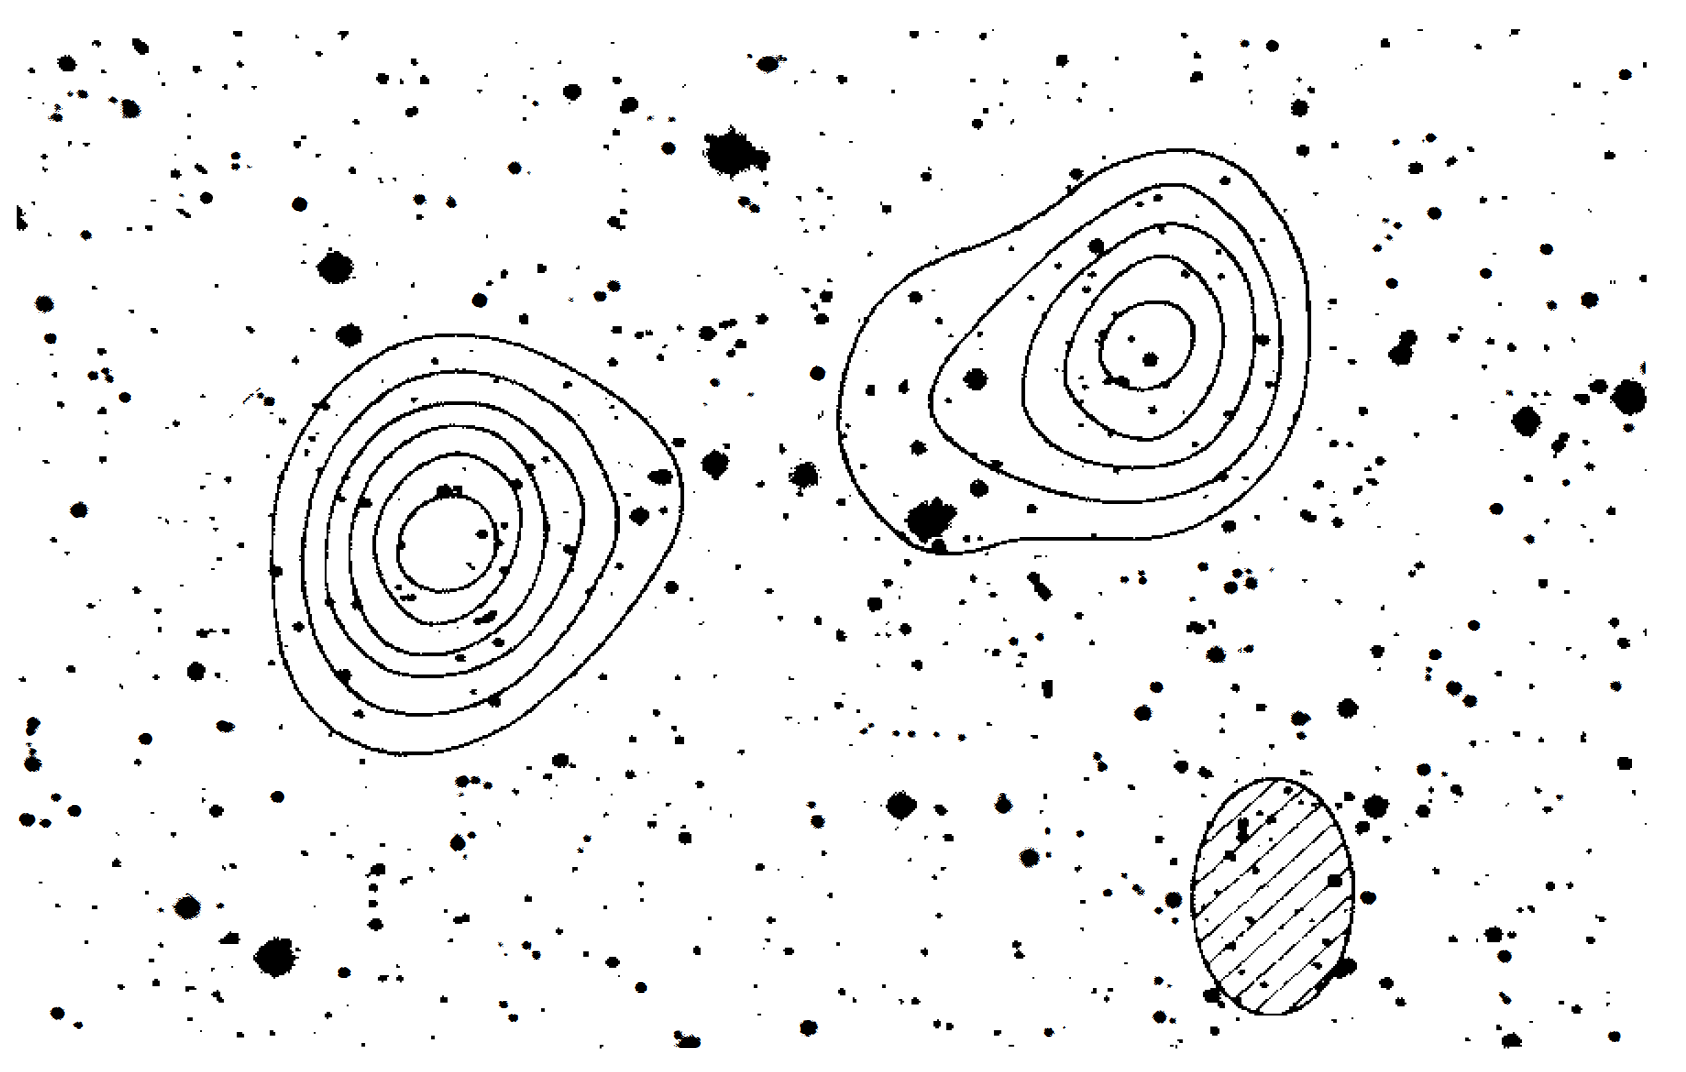
\includegraphics[width=0.9\textwidth]{plots_chp1/Cygnus_A_Hale_Baade_1965.png}}\\
  \subfloat[Cygnus A observed with the Very Large Array (VLA) at tuning frequency of $\nu_{\rm obs} = 5$ GHz \citep{CarilliBarthel1996}.]{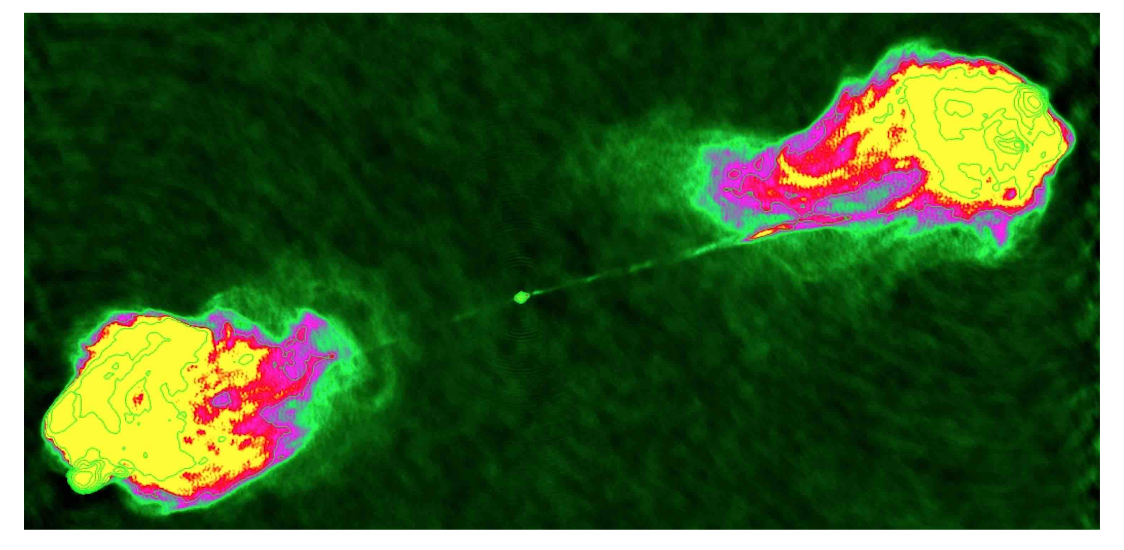
\includegraphics[width=0.9\textwidth]{plots_chp1/CygA_Carilli_Perley.png}}
  \caption[Cygnus A radio imaging in 1966 and 1996]{Radio images taken of Cygnus A in 1966 and again in 1996}
  \label{fig:CygA}
\end{figure*}

The existence of galactic scale magnetic fields is confirmed, furthermore, through the polarisation of light emitted from the AGN in a radio galaxy. With observations of polarized emission in many radio galaxies being made over the years, synchrotron radiation became increasingly plausible as an explanation for radio jet emission. Radio polarisation studies also show that polarisation increases with redshift. Generally, for sources galaxies at $z \gtrsim 0.2,$ polarisation (quantified by the rotation measure, $\rm{RM} = \int \vec{B} dl$) is relatively stronger than at lower redshift sources  \citep{Saikia1988,Scarrott1990,Tadhunter1992,Jannuzi1991,diSeregoAlighieri1993,
Tran1995,Jannuzi1995,diSeregoAlighieri1996,Jones1996,Feretti1999,Taylor2002,Kaczmarek2018}. Thus, radio polarization has been an important technique for examining the radio structures produced by jets.
 
In section \ref{section:early-radio-surveys}, I mentioned the ultra steep selection criterion for distant radio galaxies. Indeed, many studies following the work of \citet{Tielens1979}, who first displayed this bias, have shown that the radio spectral index ($\alpha$) in the relation $S_\nu \propto \nu^{-\alpha}$ correlates with redshift ($z$) \citep{BlumenthalMiley1979,Chambers1988a,deBreuck2002}. There has not been a proper consensus on the emergence of a radio spectral index and redshift anti-correlation made but several theories have been put forward. 

Radio SEDs are concave meaning that they are steeper at higher observed frequencies due to electron energy losses by inverse-Compton scattering and synchrotron radiation. This concave shape implies that at bias will be introduced where at higher redshifts, the steeper end of the spectrum where the rest frequencies are higher for a given observed frequency in radio SED. This idea only holds provided that a radio spectrum is concave which is not always the case \citep{Klamer2006}.  

More recent findings have shown that $\alpha-z$ correlation is a result of the decrease in cosmic microwave background (CMB) energy density with cosmic time. Hence, at earlier epochs the effects of Inverse-Compton scattering of CMB photons is stronger resulting in higher electron energy losses low observed frequencies ($\nu_{\rm obs} \leq$ 1 GHz). This in combination with selection effects explained in \citet{deBreuck2000} result in steeper radio spectra \citep{Morabito2018}.  

The near-infrared $K$-$z$ diagram is introduced as a motivation for studying radio galaxies in section \ref{section:motivation}. The $K$-$z$ diagram shows the $K$-band (corrected) magnitudes as a function of redshift. A $K$-band ($\lambda_{\rm c}=2.2~\mu$m) magnitude is proportional to the stellar mass of a galaxy, because it traces the more evolved stellar population. Therefore, $K$-band magnitudes are a proxy for stellar mass. The majority of $K$-$z$ diagrams assembled have shown radio galaxies to have the brightest (lowest) $K$-band magnitudes and therefore largest stellar masses of $M_*/\rm{M}_\odot \simeq 10^{10} - 10^{12}$ of all galaxy populations \citep{McCarthy1993,jarvis2001,Willott2003,rocca-volmerange2004}. The implications of radio galaxies being massive are two-fold: according to the principle of downsizing (the more massive structures form at earlier cosmic times) massive galaxies will form stars earlier during their evolution. Secondly, if their black-hole scale with their stellar masses as we known from the $M_\bullet-\sigma$ relation, we expect the AGN to expel powerful radio jets that result in kinetic feedback that could possibly shut down star-formation in as little as a few Myr. 

We mentioned earlier that radio AGN are predominantly hosted by elliptical galaxies. Some of the first evidence to emerge for this were a sample of bright galaxies drawn from the 6C catalogue \citep{Eales1985a,Eales1985b}. VLA, HST and near-IR observations of 28 radio galaxies from this sample at $0.6 < z < 1.8$ showed the stellar distributions to have elliptical morpholgies in {\it HST} imaging. Their optical, near-IR SEDs were also consistent with those of giant elliptical (gE) galaxy populations \citep{Best1997}. Further confirmation of $z \sim 1$ radio galaxies being ellipticals is put forward in \citet{McLureDunlop2000} who apply surface brightness models (Freeman Disc template and de Vaucouleurs $r^{1/4}$ Law) used on $z \simeq 0.2$ AGN to the 3CR sample and demonstrated that indeed infrared emission is dominated by starlight. They also demonstrated that the $z \simeq 0.2$ AGN hosted by elliptical galaxies and $z \sim 1$ radio galaxies may be linked via the Kormendy-relation\footnote{This is a scaling relation between the effective radius of an elliptical galaxy and its surface brightness. The bulge or low effective radius ($r_{\rm eff.}$)} zone has a higher surface brightness than the outer edges (higher $r_{\rm eff.}$) and therefore, radio galaxies evolve rather passively from $z\sim1$ to $z\sim0.2.$

At $z > 1,$ where the galaxies are often nothing but mere, unresolved point sources, determining the morphology is a tedious task. To determine the morphologies of high redshift radio galaxies, \citet{pentericci2001} attempted fitting the sources with de Vaucouleurs and exponential models to surface brightness profiles from {\it HST} and NICMOS (Near infrared Camera and Multi-Object Spectrometer). This did not lead to any meaningful conclusions pertaining to morphology. Thus, the strongest motivation for expecting an HzRG to elliptical simply lies in the notion that the progenitors of local giant elliptical population may, in fact, be HzRGs. 

Furthermore, the clumpy rest-UV sub-structures observed in the {\it HST} imaging of HzRGs at $z > 2.5$ may be evidence for dynamical instability caused by galaxy interactions and mergers \citep{pentericci2001}. 
If galaxy mergers are a trigger for AGN activity, then this may explain why higher redshift sources have such perturbed structures as well as high radio luminosities. By $z \sim 1,$ galaxies tend to be more dynamically relaxed, elliptical galaxies. Hence, given the average lifetime $\tau=10-100$ Myr radio AGN duty cycle and the dynamically perturbed optical morphologies seen in observations, it is very probable that all massive ellipticals may have passed through a period of persistent radio AGN activity at $z > 2.5.$ 

The more dynamically relaxed radio galaxies at low-$z$ are observed as optically red hence quiescent with low levels of ongoing star-formation. These observed characteristics as well as the tightness of Hubble $K$-$z$ relation suggest that HzRGs may be progenitors of local radio galaxies \citep{Stanford1998}. Further evidence in support of this is given by observations of 3CR radio galaxies which commonly reside in over-dense or rich cluster or group environments at $z \sim 1$ \citep{Yates1989,HillLilly1991,Best2000b}. However, the environments of FR II type galaxies are rich clusters at higher reshifts and smaller groups at low-$z.$ If HzRGs evolved into local radio galaxies, there would be no discrepancy between their observed environments, perhaps. This, therefore, suggests that rather HzRGs and local radio follow disparate evolutionary tracks \cite{Best1998b}. 

Despite sharing similar observational characteristics, HzRGs may only be the progenitors of local galaxies, in a few cases. This is suggested somewhat by radio galaxies at $z \gtrsim 1$ which have extended emission line gas haloes, clumpy UV sub-structures and the radio-optical alignment that are observed less so or not at all in nearby radio galaxies. We can, thus, think of low-$z$ radio galaxies and high redshift radio galaxies (HzRGs) as discrepant populations, evolutionarily that happen to share a few common observed characteristics.  

\section{High-redshift radio galaxies (HzRGs)}  
High-redshift radio galaxies are found at $z > 1.$ As mentioned in section \ref{section:early-radio-surveys}, some of the first identifications of very distant radio galaxies. The 4C sample observed at 178 MHz with a flux limit of $S_{178}=2$ Jy, in particular led, to the observation of 35 distant radio galaxies with steep spectral indices, $\alpha < -1$ via the ultra-steep spectrum (USS) method resulting in the 4C/USS sample at $\nu_{\rm obs} \leq 1$ GHz \citep{ChambersMiley1990}. In the wake of this study, the USS method became the primary detection method for detecting HzRGs which have rather distinct characteristics. 

% Radio-optical alignment
One of these is the observed alignment effect. HzRGs are characterised by rest-UV and optical emission which, as mentioned before, tends to be clumpy rather than homogenous. These inhomogeneities are observed within the inner regions of the gas halo leading to the assumption that they kinematically perturbed by turbulent gas motions around the AGN where rapid accretion occurs. Furthermore, in many HzRGs, the rest-UV and optical emission tends to be very well aligned with the radio axes (the projected orientation of the relativistic jets)\citep{Djorgovski1987,McCarthy1987b,Chambers1988b}. Explanations cited for the alignment effect have been jet-induced star-formation \citep{Rees1989,Bicknell2000}. The passage of radio jets shock excites dense molecular clouds resulting inducing local instabilities required for the gas clouds to collapse and form stars. 

% Protocluster environments
Another distinct characteristic of HzRGs is their galactic environments. HzRGs are primarily located in early and forming galaxy clusters referred to as {\it proto-clusters}. One distinguishing characteristic of proto-clusters is the over-density of Ly$\alpha$ $\lambda1215$ emitters that are detected within them, up to Mpc distance-scales. Evidence of this has been given by extensive Ly$\alpha$ narrow band imaging carried out with the aim of finding these early clusters. Some examples of this are the proto-clusters discovered at $2.2 < z < 5.2$ with the unit telescopes of the Very Large Telescope (VLT) \citep{Kurk2000,Venemans2002,Venemans2004,Croft2005}. Other important facilities used to discover proto-clusters have been {\it HST} as well as the {\it Spitzer Space Telescope} \citep{Miley2004,Overzier2005,Kodama2007,Galametz2010,Galametz2012}. These studies have managed to demonstrate that within fields of up to $\sim3$ Mpc, HzRG environment are sprawling with Ly$\alpha$ emitters \citep{Venemans2007}. These observations distinguish HzRGs from radio galaxies at $z\sim0.5$ where only 50\% of radio-loud AGN host galaxies reside in rich clusters \citep{HillLilly1991}. 

% Relevance of HzRGs within context of galaxy evolution
Since the discovery of HzRGs via the USS method, these sources have been fundamental in answering important questions pertaining to the evolution of galaxies that host radio-loud cores. Some pressing questions, however, still remain. What is the main cause of the rest-UV/optical alignment? What ionises the warm gas medium: star-formation or radiation from the AGN or both? Where is the neutral HI gas within the haloes of these galaxies? How do jet interact with the surrounding ISM and what affect does this have on star-formation? 

I trust that upcoming radio surveys will be a cornerstone in answering some of these puzzling questions. HzRG observations will be thoroughly improved with the advent of new telescopes and instrumentation. Future radio interferometers such as the uGMRT (upgraded Giant Metrewave Radio Telescope), MeerKAT and the SKA (Square Kilometer Array), and others of this calibre will be of great importance in this matter. The upcoming instruments will have the capability to detect radio sources at new and unprecedented flux limits yielding radio continuum imaging and polarization maps that will provide the data needed for studies of radio galaxies near and far. 

\bibliographystyle{mnras}
\bibliography{intro_1_2}

\end{document}